\documentclass[12]{article}
\usepackage{times}
\usepackage{natbib}
\usepackage{multicol}
\usepackage{hyperref}

\usepackage{amsmath, amssymb, fullpage, amsthm, array, algorithm2e,graphicx,mathtools, xparse}

\usepackage{color}
\usepackage{subfigure}
%\usepackage[dvips]{graphics}
\newtheorem{thm}{Theorem}[section]
\newtheorem{dfn}{Definition}[section]
\newtheorem{cor}{Corollary}[thm]
\newtheorem{con}{Conjecture}[thm]
%\setlength{\parindent}{0in}   % for no indent

\topmargin -0.10in   % when making pdf
\textheight 8.5in  % when making pdf

\begin{document}


%% ================ chapter 2 starts here  ==========================

\title{Visual Statistical Inference for Large $p$, Small $n$ Data}\label{ch:largepsmalln}
\vspace{-0.8cm}
\author{Niladri Roy Chowdhury, Dianne Cook, Heike Hofmann, Mahbubul Majumder}
%\large{This paper was presented in Joint Statistical Meetings 2011 and is submitted in JSM Proceedings 2011.} 

%\vspace{1cm}

%\normalsize

\maketitle

\begin{abstract}
Statistical graphics plays an important role in exploratory data analysis, model checking and diagnosis. Recently there were some formal visual methods for determining statistical significance of findings. We often seek to low-dimensional projections in high dimensional data which reveal important aspects of the data. Projection pursuit for classification finds projections that reveal differences between classes. In this paper we are interested in the performance of classification methods when the number of observations is relatively small compared to the number of variables, known as a large $p$ (dimension) small $n$ (sample size) problem using visual statistical inference. We apply projection pursuit for classification to pure noise data and to the data when there is some separation. We use the lineup protocol \cite{buja:2009} to make comparisons among the pure noise data and the data which has some separation.

\end{abstract}

\section{Introduction} 
%testing

%topic
{\color{green} History of visualization. Why statistical graphics is important.}

Any statistical analysis must include some statistical graphics. For exploratory data analysis, statistical graphics play an invaluable role in model checking and diagnostics. Even though we have established mathematical procedures to obtain various statistics, we need to support the results by also producing the relevant plots. \\
%topic
{\color{green} Recent advancements in statistical graphics. How statistical graphics has been recently used as a tool for statistical inference.}\\
In recent times there have been major advances in statistical graphics. Modern computing systems like R and SAS produce high quality statistical graphics. \cite{buja:2009}, following from Gelman [2004], proposed two protocols that allow the testing of discoveries made from statistical graphics. \\
%topic
{\color{green} Explanation of Projection Pursuit.} \\
In this paper we used the idea of projection pursuit by Friedman and Tukey [1974]. Projection pursuit is a statistical tool to find the most interesting projections from high dimensional to low dimensional space that reveals the most details about the structure of the data. In this paper we mainly use the one and two dimensional projections obtained by projection pursuit on higher dimensions. \\
%topic
{\color{green} Explanation of \texttt{tourr} package.} \\
In this paper we use the \texttt{tourr} package in \texttt{R} \cite{r} by \cite{WC08}. 

The \texttt{tourr} package produces tours of multivariate data. The package also includes functions for creating different types of tours like grand, guided and little tours, which project multivariate data with $p$ dimensions to 1, 2, 3 or $d$ dimensions where $d \le p$. In this paper we mainly use the guided tour function which instead of picking a new projection completely at random, it picks projections that are closer to the current projection, so that we eventually converge to a single maximally interesting projection. The \texttt{tourr} package comes with 4 indices but we use the PDA (Penalized Discriminant Analysis)  index described in \cite{lee:2009}. \\     
%topic
{\color{green} Outline of the different sections.}\\
In this paper we check the projection pursuit optimization on pure noise with no real separation by using statistical graphics in Section \ref{sec:largep}. We also check the PP optimization on dimensions with some real separation and present results. In Section  \ref{sec:distance} we are also concerned about how the distance between the means increase with $p$ for a fixed n. We also present a probable range for the number of dimensions at which the clusters starts to separate out for both one dimensional and two dimensional projections.

%\section{Visual Statistical Inference} \label{sec:visual_test} 
%
%This section outlines the concepts of visual inference in comparison to the procedures of classical statistical inference. 
%
%Let $\theta$ be a population parameter of interest, with $\theta \in \Theta$, the parameter space. 
%Any null hypothesis $H_0$ then partitions the parameter space into $\Theta_0$ and $\Theta_0^c$, with $H_0: \theta \in \Theta_0$ versus $H_1: \theta \in \Theta_0^c$. 
%% In hypothesis testing terminology, the parameter space $\Theta$ of a population parameter $\theta$, can be partitioned into $\Theta_0$ and $\Theta_0^c$. We test $H_0: \theta \in \Theta_0$ versus $H_1: \theta \in \Theta_0^c$.
%
%%\subsection{Visual Statistic} 
%
%Unlike classical hypothesis testing, the statistic in visual inference is not a single value, but a plot that is appropriately chosen to describe the parameter of interest, $\theta$. When the alternative hypothesis is true, it is expected that the plot of the observed data, the test statistic, will have visible feature(s) consistent with $\theta \in \Theta_0^c$, and that visual artifacts will not distinguish the test statistic as different when $H_1$ is not true.
%
%\begin{dfn}\label{dfn:lplot}
%A lineup plot is a layout of $m$ visual statistics, consisting of 
%\begin{itemize}\itemsep-3pt
%\item $m-1$ plots simulated from the model specified by $H_0$  (null plots) and 
%\item the test statistic produced by plotting the observed data, possibly arising from $H_1$.
%\end{itemize}
%\end{dfn}
%
%If $H_1$ is true, the test statistic is expected to be the plot that is most different from the other plots in the lineup plot. A careful visual inspection should reveal the differences in the feature shown by the test statistic under null and alternative hypothesis. {\em If the test statistic cannot be identified} in the lineup, the conclusion is to {\em not reject the null hypothesis.} The $(m-1)$ null plots can be considered to be samples drawn from the sampling distribution of the test statistic assuming that the null hypothesis is true.
%
%
%Since the lineup plot consists of $m$ plots, the probability of choosing any one of them is $1/m$. Thus we have type-I error probability of $1/m$.
%
%The lineup plot can be evaluated by one or more individuals. When a single individual identifies the observed graph in the lineup plot we report a $p$-value smaller than $1/m$, otherwise the $p$-value is larger than $1/m$. 
%
%If $N$ individuals evaluate a lineup plot independently, we count the number of successful evaluations as $U \sim \text{Binom} (N,\frac{1}{m})$ and report a  $p$-value of at most $Pr(U \ge u)= \sum_{k \ge u}^N {{N \choose k} (\frac{1}{m})^k(1-\frac 1m)^{(N-k)}}$ where $u$ is the observed number of successful evaluations. %Notice that when $N=1$, this $p$-value is $\frac1m$. 
%
%
%For two different visual test statistics of the same observed data, the one  is better, in which a specific pattern is more easily distinguishable visually.

\section{Inference for the means of two populations} \label{sec:largep}
%\section{Checking PP Optimization} \label{sec:largep}

\subsection{Motivation}
%topic
{\color{green} Statement of the problem. What we want to show. }\\
Consider two random samples $X_{i1}, X_{i2}, \dots, X_{ip}$ for $i = 1$ and 2 which have means $\mu_1 = (\mu_{11}, \mu_{12}, \dots, \mu_{1p})^T$ and $\mu_2 = (\mu_{21}, \mu_{22}, \dots, \mu_{2p})^T$ respectively. We consider testing the following high-dimensional hypothesis :

$$H_0 : \mu_1 = \mu_2 \qquad \hbox{versus} \qquad H_a : \mu_1 \neq \mu_2 .$$

The hypothesis $H_0$ consists of the $p$ marginal hypotheses $H_{0l} : \mu_{1l} = \mu_{2l}$ for $l = 1, \dots, p$ regarding the means on each data dimension.

%The optimization procedure in the  \texttt{tourr} package is new, different from the algorithms that have existed before in GGobi \cite{STLBC03} and XGobi \cite{SCB91}. 
%We have been using PP with the PDA index, on a large $p$, small $n$ data set from a microarray study, and for comparison have been looking at pure noise data. As strange as it might seem it seemed like we could often pick the projection of the  ``original'' data from a lineup of projections of permuted class data. This should not be possible. 

\subsection{Procedure}
%topic
{\color{green} Description of the procedure. }\\
For testing the above hypothesis, we simulate two sets of $p$-dimensional data from a standard normal distribution with $n = 15$ observations in each dimension in each set. Consider $Z_{ij} = (Z_{i1}, Z_{i2}, \dots, Z_{ip})$ for $i = 1$ and 2 and $j = 1, \dots, p$ are simulated from a $N(0, 1)$ distribution. These  two sets of data should represent the random samples collected from the two population. To test for the equality of means, we bring in some separation in the last dimension by adding and subtracting a value $\delta$ from the mean of the dimensions.  

We define $X_{1p} = - \delta + Z_{1p} $ and $X_{2p} = \delta + Z_{2p}$. 
We bring in a class variable which indicates the population the dataset is obtained from. The first 15 observations are labeled class 1 and the second 15 observations are labeled class 2.  We compute projection pursuit using the PDA index and plot the one dimensional projections in a lineup plot with $m=20$ where alternatives plots are created by randomly permuting the class labels.  We showed the lineup plots to several subjects and asked them to identify the plot which has the largest separation among the groups.

To compare the above method, we again simulate two sets of $p$-dimensional data from a standard normal distribution with $n = 15$ observations in each dimension in each set. So now we have $X_{ij} = Z_{ij}$ for $i = 1$ and 2 and $j = 1, \dots, p$. So the two datasets from the two population do not have any real separation and they are pure noise. We again compute using the PDA index and plot the one dimensional projections in a lineup plot with $m=20$ where alternatives plots are created by randomly permuting the class labels. Several individuals were again asked to identify the plot which has the largest separation among the groups.\\[1cm]


{\color{blue}Do not know how to write the two dimensional projections in this set up. May be test for equality of mean vectors for 3 populations ??}

%There is no true class, it is pure noise data -- any separation seen between classes in the projection are purely due to the high dimension.
%We expect that the original data should not be detectable -- it's just noise, any labeling of the observations to class is random. 

%For 2D projections data is simulated from a standard normal distribution with $n=30, p=100$. The first 10 observations are labeled class 1, the second 10 observations are labeled class 2 and the last third are labeled class 3. There is no true class, it is pure noise data. To account for the occasional convergence problem with the optimization 30 null plots are generated. The 19 null plots which have the smallest Wilks $\lambda$ (\cite{JW02}) values are used for the lineup. 
%
%For comparison, for each of these examples we also simulated data that had real classes, too. We also simulated data with 99 dimensions of pure noise and one dimension of real separation, in all making it 100 dimensions. In the same way, each dimension has 30 observations and they were divided into 2 classes. The separation was designed in a way such that if we plot the one dimension with real separation, the points lie approximately 6 units apart. Once again the first 15 observations are labeled class 1 and the last 15 observations are labeled class 2. In this case there is one dimension of real separation. We once again compute the projection pursuit using the PDA index and plot the one dimensional projections.
%
%For 2D projections, data is simulated 100 dimensions of pure noise. Again each dimension has 30 observations with 3 classes. But in this case the last two dimensions are changed so that the data has some real separation. The two dimensions with real separation was constructed such that the points lie close to the vertex of an equilateral triangle of side 6 units. Once again the first 10 observations are labeled class 1, the second 10 observations are labeled class 2 and the last third are labeled class 3. Here we have two dimensions of real separation. We again compute projection pursuit using the PDA index and plot the two dimensional projections in a lineup plot.  To account for the occasional convergence problem of optimization we select the 19 plots with the minimum Wilk's $\lambda$ from the generated 30 plots generated.
%
%Figure \ref{fig:test_category_1d} gives the lineup plot for the one dimensional projections for 100 dimensions of pure noise and Figure \ref{not_noise_1d} gives the lineup plot for the one dimensional projections for 99 dimensions of pure noise and 1 dimension of real separation.
%
%Figure \ref{fig:test_category} gives the lineup plot for the two dimensional projections for 100 dimensions of pure noise and Figure \ref{not_noise} gives the lineup plot for the two dimensional projections for 98 dimensions of pure noise and 2 dimensions of real separation.

%\end{multicols}
%
\begin{figure}[hbtp]
%\begin{figurehere}
   \centering
       \scalebox{1.00}{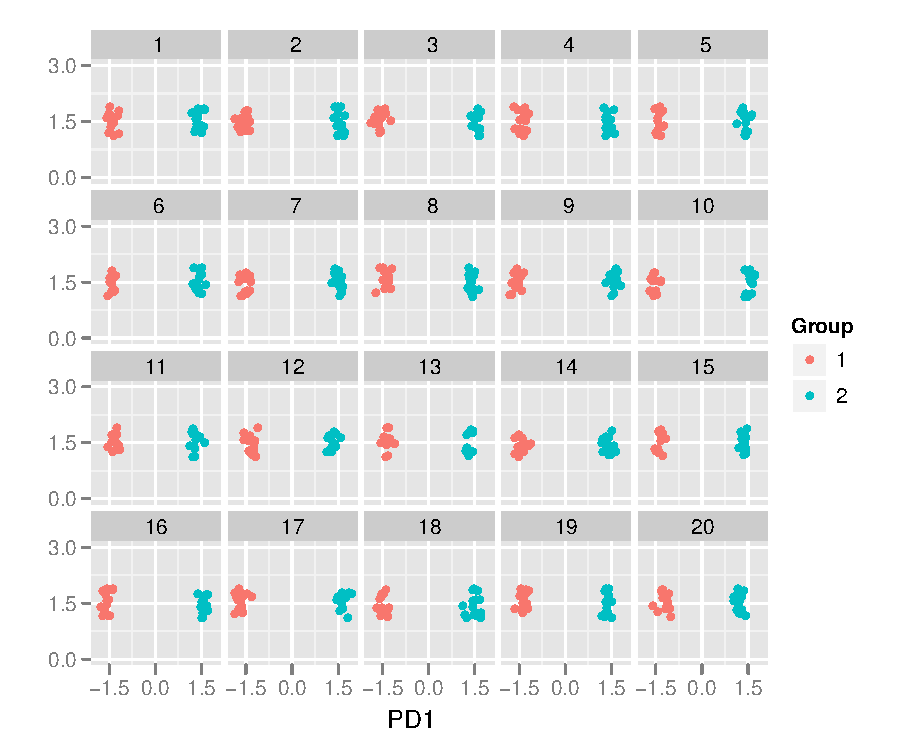
\includegraphics{plot_1d_100_4.pdf}}
       \caption{Lineup plot ($m=20$) with 100 dimensions of random noise for testing $H_0$: There is no difference among the plots. When the alternative hypothesis is true the observed plot should have the largest separated colors. Can you identify the observed plot?}
     \label{fig:test_category_1d}
%\end{figurehere}
\end{figure}
%
%
\begin{figure}[hbtp]
%\begin{figurehere}
   \centering
       \scalebox{1.00}{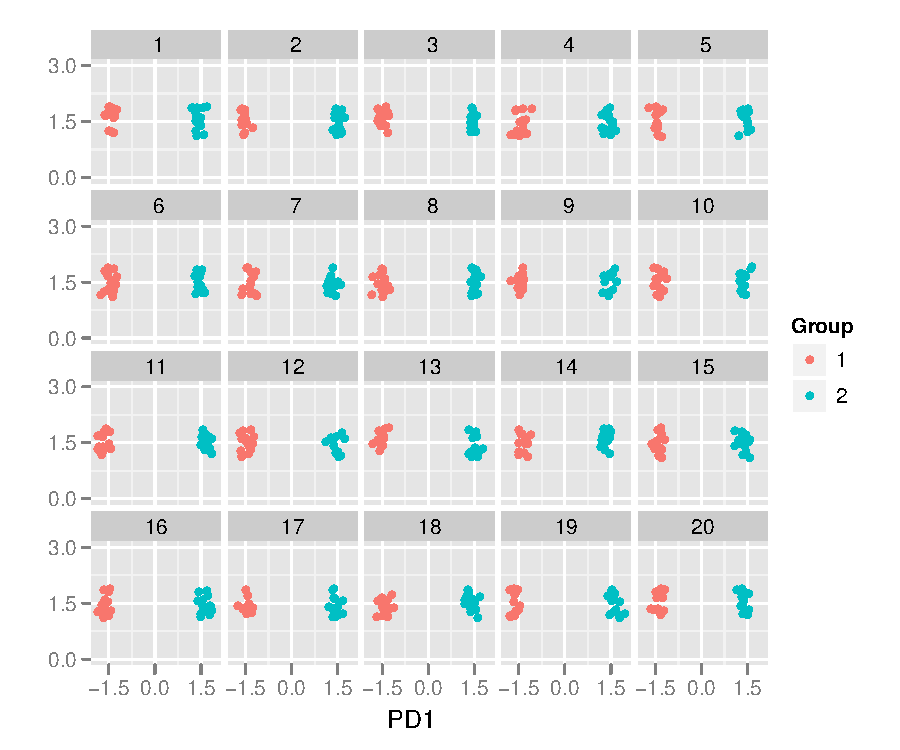
\includegraphics{plot_1d_99_19.pdf}}
       \caption{Lineup plot ($m=20$) with 99 dimensions of pure noise and 1 dimension of real separation for testing $H_0$: There is no difference among the plots. When the alternative hypothesis is true the observed plot should have the largest separated colors. Can you identify the observed plot?}
       \label{not_noise_1d}
\end{figure}
 
%\begin{figure}[hbtp]
%%\begin{figurehere}
%   \centering
%       \scalebox{1.00}{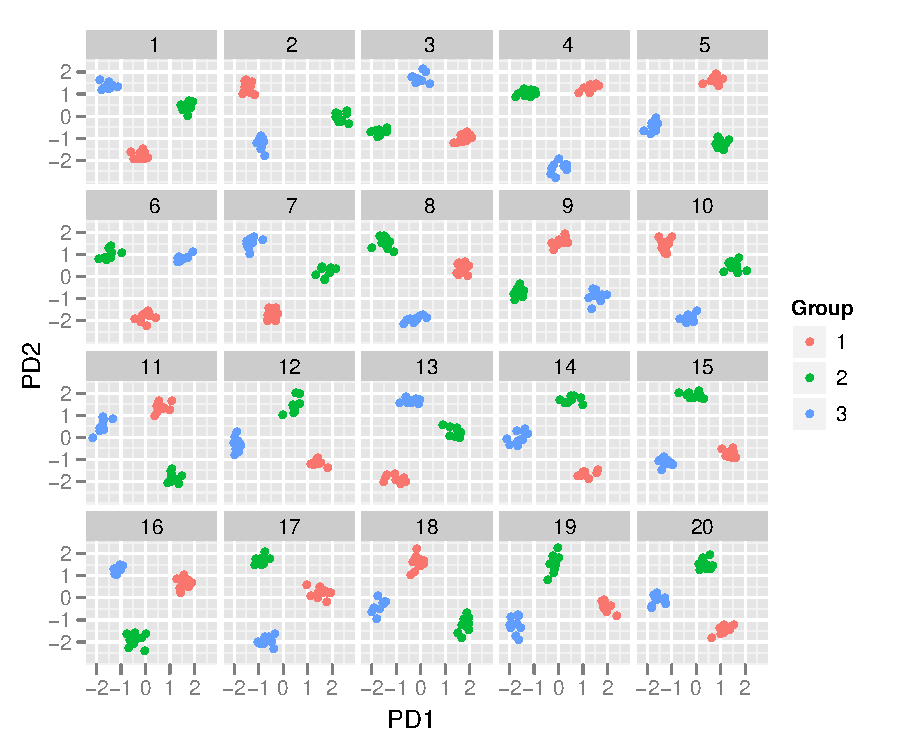
\includegraphics{plot_2d_100_15.pdf}}
%       \caption{Lineup plot ($m=20$) with 100 dimensions of random noise for testing $H_0$: There is no difference among the plots. When the alternative hypothesis is true the observed plot should have the largest separated colors. Can you identify the observed plot?}
%       \label{fig:test_category}
%%\end{figurehere}
%\end{figure}
%
%
%\begin{figure*}[hbtp]
%%\begin{figurehere}
%   \centering
%       \scalebox{1.00}{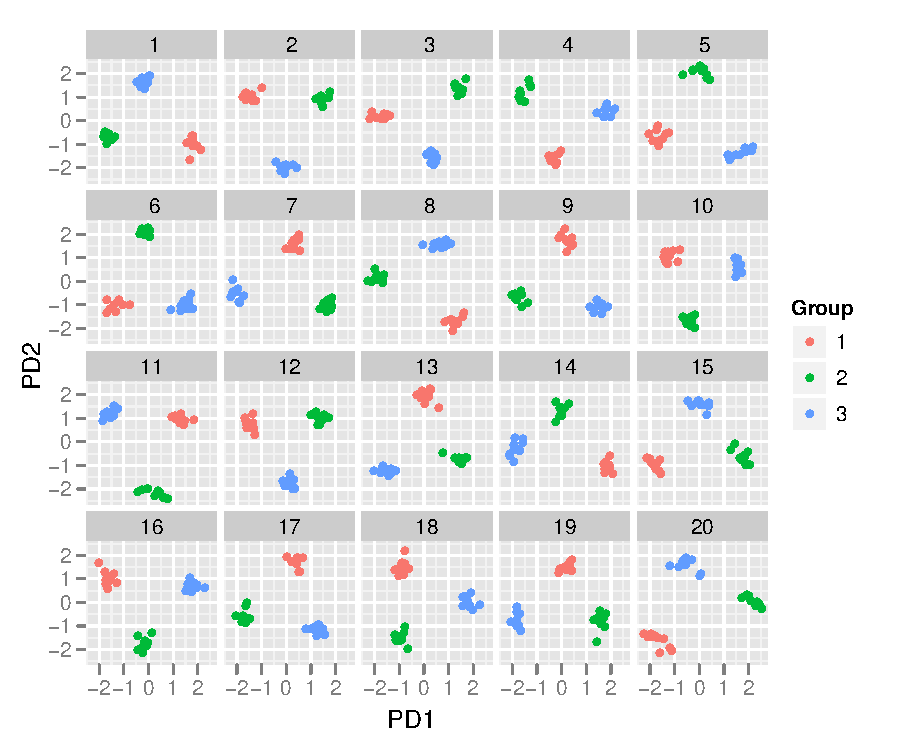
\includegraphics{plot_2d_98_5.pdf}}
%       \caption{Lineup plot ($m=20$) with 98 dimensions of pure noise and 2 dimensions of real separation for testing $H_0$: There is no difference among the plots. When the alternative hypothesis is true the observed plot should have the largest separated colors. Can you identify the observed plot?}
%       \label{not_noise}
%\end{figure*}

%\begin{multicols}{2}

\subsection{Results}
%topic
{\color{green} Description of the experiment. How the experiment was conducted. What are the parameters, how many different plots.} \\
An experiment is designed to study the ability of human observers to detect the effect of one dimension of real separation in $p$ dimensions of noise. Data is simulated for different values of $p$  ( = 20, 40, 60, 80, 100) with sample size $ n  =  15$. For bringing in the real separation, we fixed $\delta $ = 3. So two sets of $p$ dimension of data with sample size $n = 15$ were generated from Normal(0 ,1) for the two populations.  $\delta = 3$ was added and subtracted to the $p$-th dimension to bring in the largest separation.  We also repeated the above procedure for the different $p$ dimensions of pure noise with no real separation ($\delta = 0$). Data sets with different combinations of $n$, $p$ and presence of noise were generated with frequencies shown in Table \ref{freq}. Three replicates of each level were generated.These produced 30 different ``observed data sets". ({\color{blue} only for one dimensional projections.}) 

\begin{table}[htbp]
\begin{center}
\caption{Values of parameters considered for the experiment.}
\begin{tabular}{cccp{3cm}}
  \hline
  \hline
  $n$ & projection & presence of real separation & $p$ \\
  \hline
  15 & 1 & Y & 20, 40, 60, 80, 100 \\
      & & N & 20, 40, 60, 80, 100\\
 %    10 & 2 & Y & 20, 40, 60, 80, 100 \\
  %    & & N & 20, 40, 60, 80, 100\\   
      \hline
\end{tabular}
\label{freq}
\end{center}
\end{table}
%topic
{\color{green} How the null plots were generated. }\\
The 19 null plots in the lineup were obtained by  permuting the population indicator variable (the variable that indicates which population the data set belongs to) so that breaking any dependency between the indicator variable and the other variables. Two different statistics Wilk's $\lambda$ (\cite{JW02})  and the within sum of squares to between sum of squares ratio were calculated for each of the 20 plots in the lineup. \\
{\color{green} The data recorded for the participants. How many participants were recruited.} \\
Participants  for the experiment were recruited through Amazon Mechanical Turk. Each participant was shown a sequence of 9 lineups. They were asked to identify the plot which has the most separation between the colored groups, give a reason for their choice and determine the level of confidence for their decision.  Gender, age, educational qualification and location of each participant were also noted. In total, 1137 lineups were evaluated by 103 participants from different locations. \\

%topic
{\color{green} Description of the results. }\\
\begin{figure*}[hbtp]
%\begin{figurehere}
   \centering
       \scalebox{0.80}{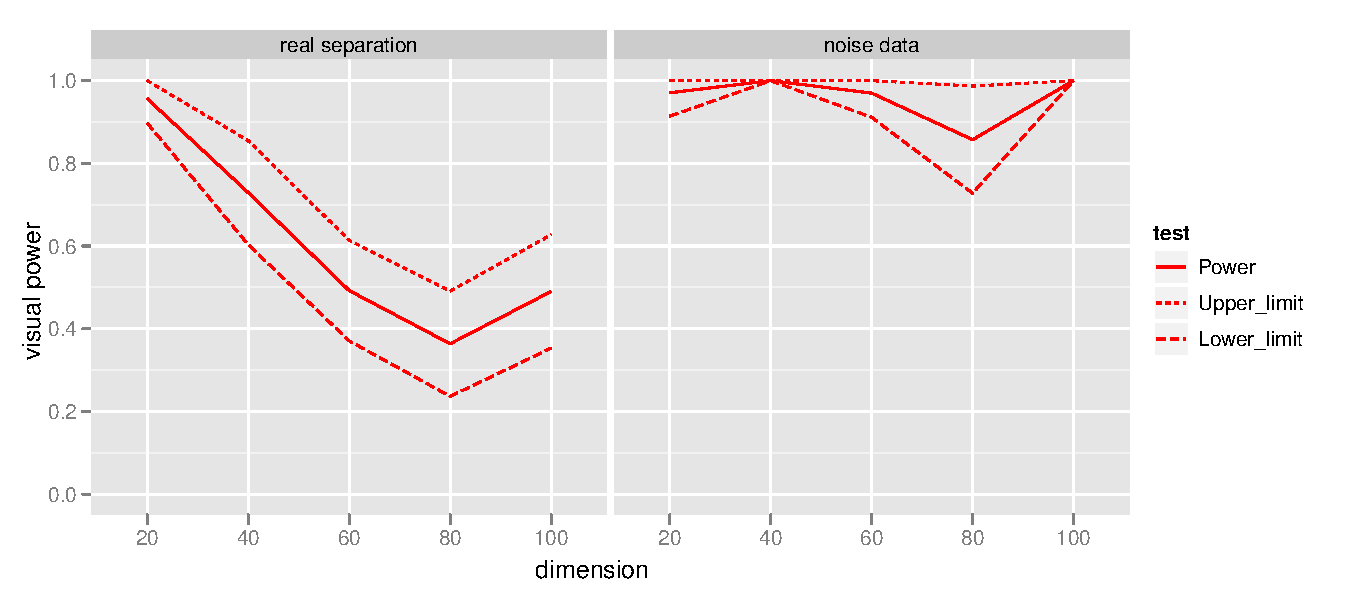
\includegraphics{power-1d.pdf}}
%       \caption{Lineup plot ($m=20$) with 98 dimensions of pure noise and 2 dimensions of real separation for testing $H_0$: There is no difference among the plots. When the alternative hypothesis is true the observed plot should have the largest separated colors. Can you identify the observed plot?}
%       \label{not_noise}
\end{figure*}

\Large{\textit{What affects the decision of the people?}} \\[0.2cm]

\normalsize
%topic
{\color{green} What do people see when they select a plot.} \\
Participants were asked to identify the plots which has the most separated colored groups. In data sets with real separation, participants make mistakes in picking up the plot of the ``observed data". The Wilk's $\lambda$ value of the plots reveal that in most situations, the plots chosen by the participants have the smallest Wilk's lambda value and hence the largest separation among the groups. This happens although the population indicator variable is permuted and any dependence between the indicator variable and the other variable is broken. So we obtain a smaller Wilk's $\lambda$ value in a null plot than the observed plot with some real separation. Figure \ref{wilks-count} shows the count of each plot by the corresponding Wilk's $\lambda$ value. 

\begin{figure*}[hbtp]
%\begin{figurehere}
   \centering
       \scalebox{0.80}{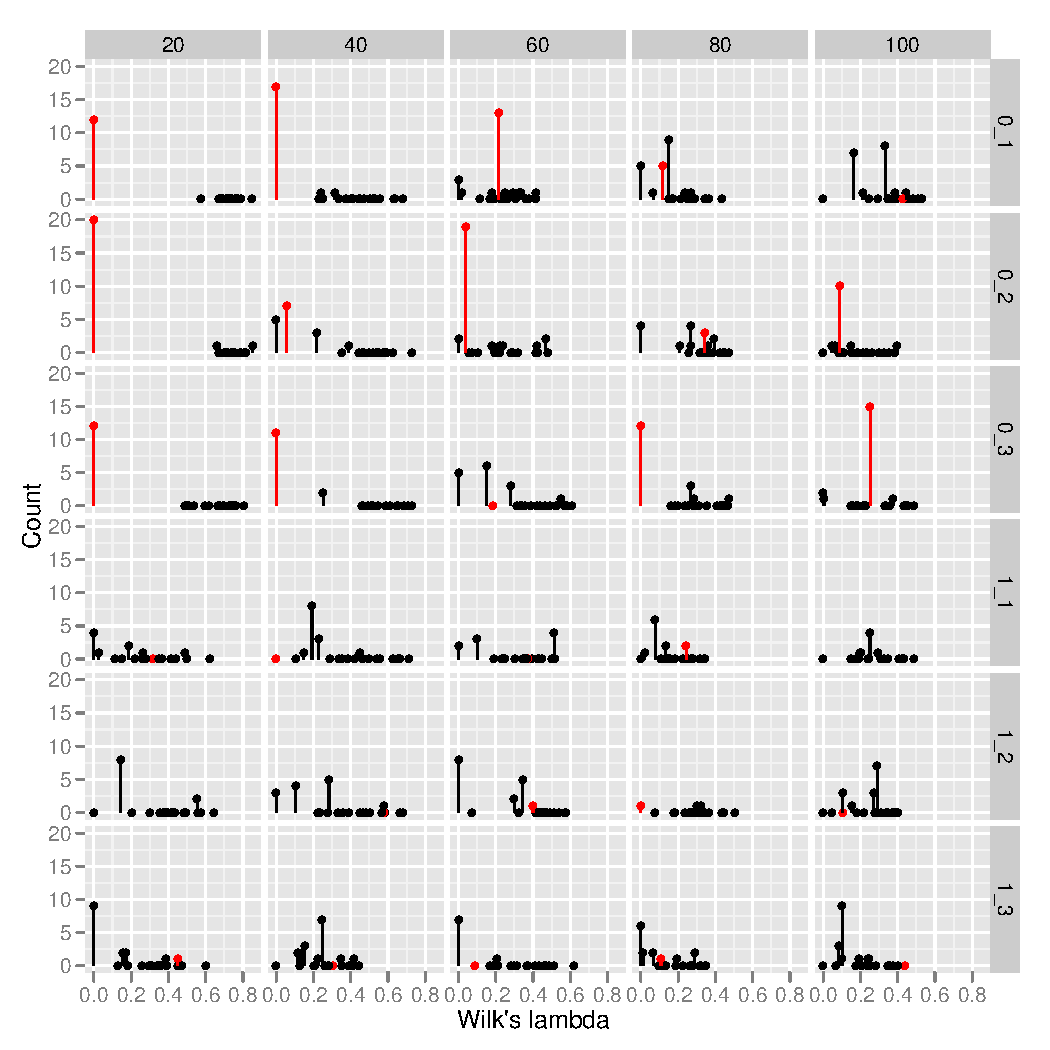
\includegraphics{wilks-count-1d.pdf}}
%       \caption{Lineup plot ($m=20$) with 98 dimensions of pure noise and 2 dimensions of real separation for testing $H_0$: There is no difference among the plots. When the alternative hypothesis is true the observed plot should have the largest separated colors. Can you identify the observed plot?}
       \label{wilks-count}
\end{figure*}

%We made 5 lineups of each of the above plots for each dimension and showed to different individuals. They were asked to pick up the ``true" one among the 20 plots. By the ``true" one, we meant the one with the most separated colors. 20\% of the individuals could identify the true plot when the data is 100 dimensions of pure noise for one dimensional projections. But when there is one dimension of separation in 100 dimensions of pure noise, 90\% of the individuals could successfully identify the true plot. For the two dimensional projections, only 30\% of the individuals could identify the true plot when the data has 100 dimensions of pure noise but 60\% of the individuals can pick the correct plot when there is two dimensions of real separation. It is evident that people are mostly correct in selecting the true plot when one dimension among 100 dimensions have real separation. People are also correct to pick the plots when two dimensions among 100 have real separation.



%\subsection{Comparisons with real separation}
%
%We also created plots with 99 dimensions of pure noise and one dimension of real separation, in all making it 100 dimensions. In the same way, each dimension has 30 observations and they were divided into 2 classes. The separation was designed in a way such that if we plot the one dimension with real separation, the points lie approximately 6 units apart. For plotting the two dimensional projections, we considered 98 dimensions of pure noise and 2 dimensions of real separation. Again each dimension has 30 observations with 3 classes. The two dimensions with real separation was constructed such that the points lies close to the vertex of an equilateral triangle of side 6 units.
%
%We made 5 lineups of such plots for each dimension and showed them to the same individuals. They were again asked to pick the plot with the most separated colors. The proportion of correct choices were 0.9 and 0.6 respectively for the one and two dimensional projections. Figure \ref{fig:result} shows the proportion of correct response by pure noise only or presence of known real separation. It is evident that people are mostly correct in selecting the true plot when one dimension among 100 dimensions have real separation. People are also correct to pick the plots when two dimensions among 100 have real separation.

%\end{multicols}

%\begin{figure}[hbtp]
%%\begin{figurehere}
%   %\centering
%       \centerline{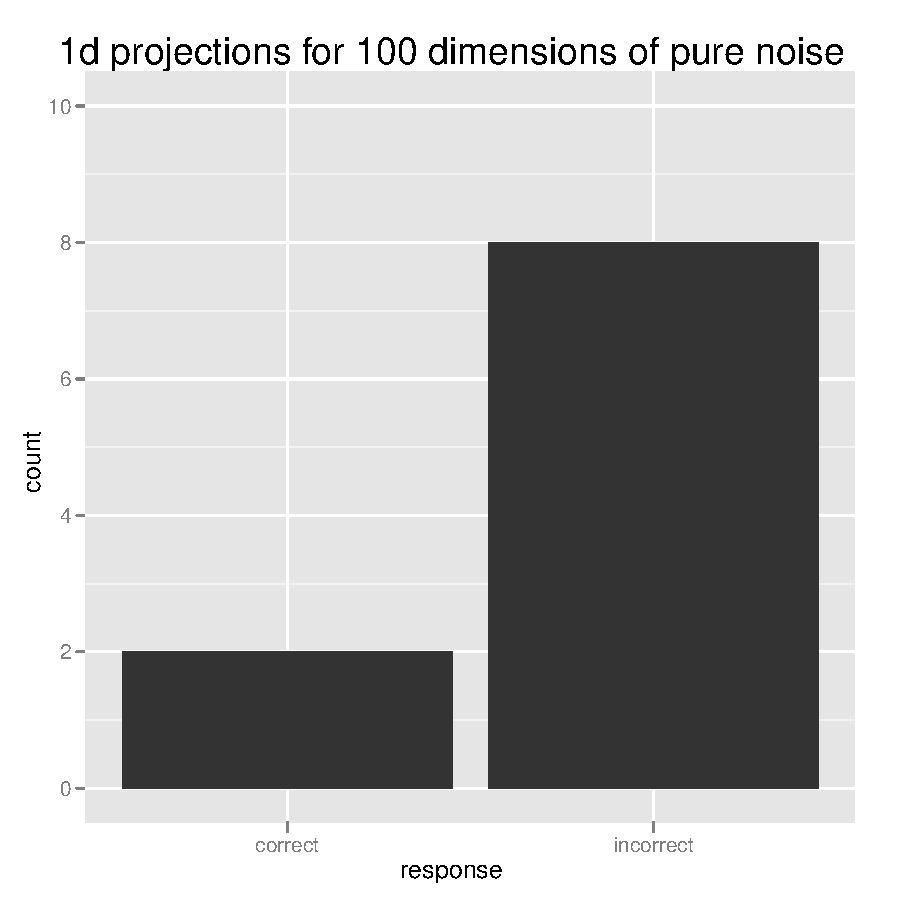
\includegraphics[width=0.25\textwidth]{result_1d_noise.pdf}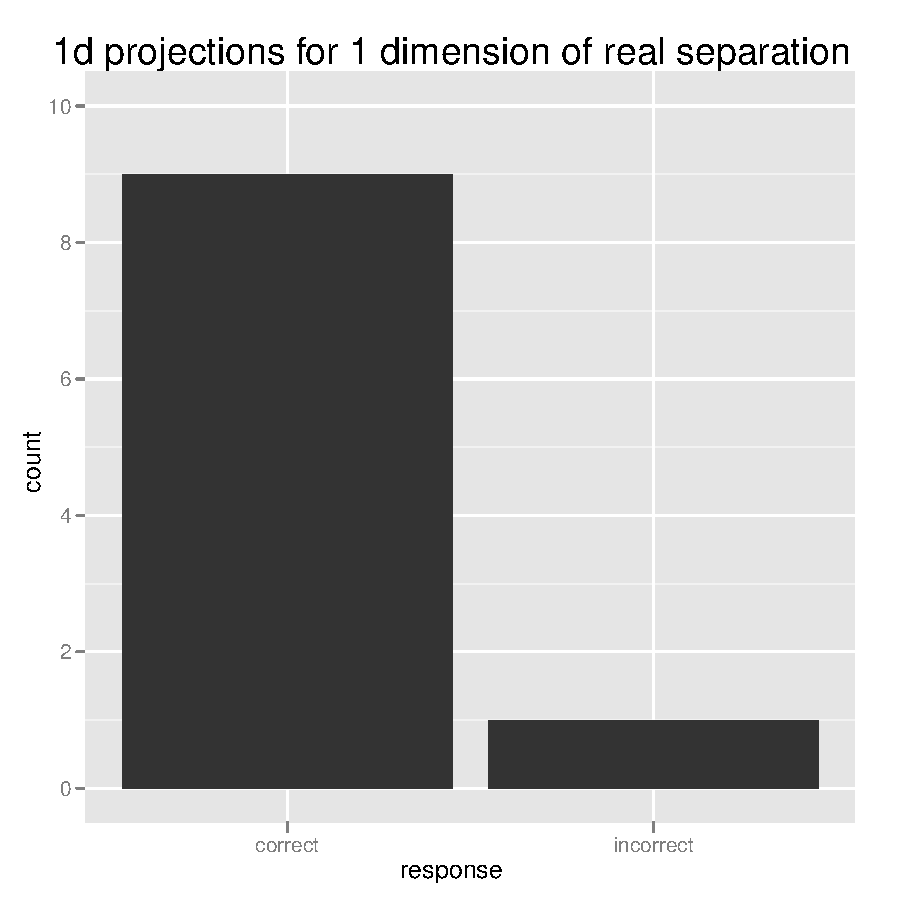
\includegraphics[width=0.25\textwidth]{result_1d_sep.pdf}}
%       \centerline{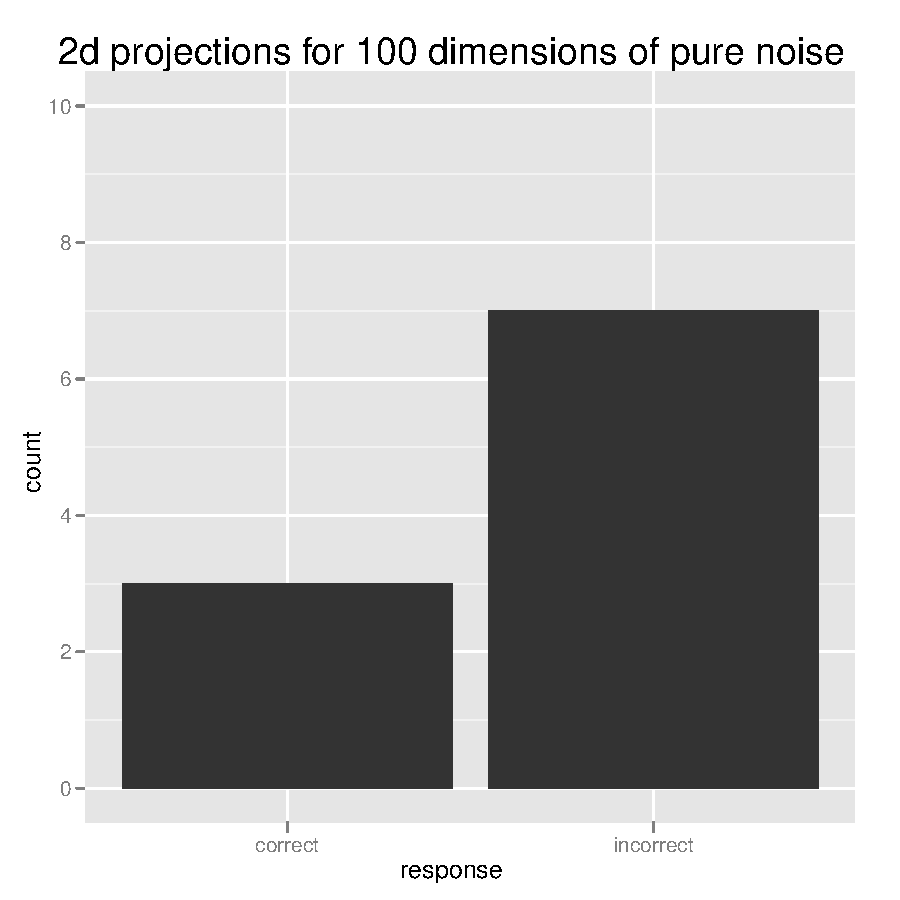
\includegraphics[width=0.25\textwidth]{result_2d_noise.pdf}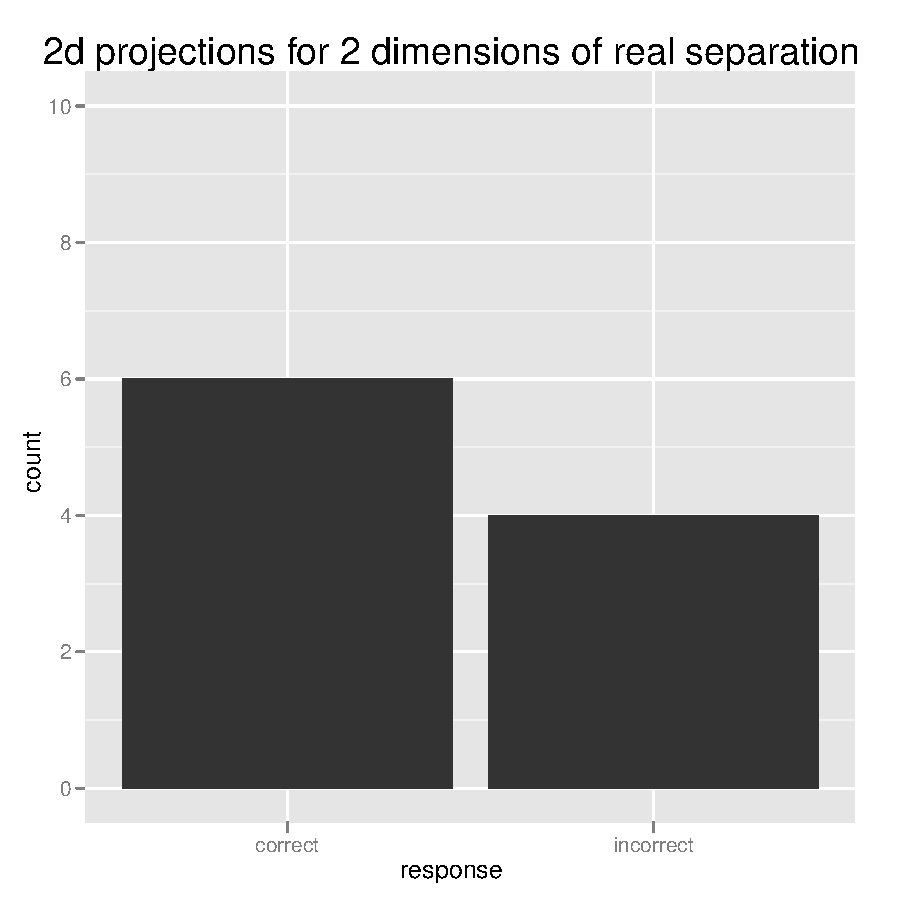
\includegraphics[width=0.25\textwidth]{result_2d_sep.pdf}}
%       \caption{Barplots showing the number of correct responses for one and two dimensional projections for data with pure noise and data with real known separation. People are more often correct in selecting the true plot when there is some real separation.  }
%       \label{fig:result}
%\end{figure}
%%\end{figurehere}



%\begin{multicols}{2}





\section{Distance Increasing with $p$ for Fixed $n$} \label{sec:distance}

\subsection{Procedure}
%topic
{\color{green} Description of the procedure to look at the distance between the groups as we increase the number of dimension for a data with no real separation.} \\
Consider two dimensions of pure noise, each dimension having 30 observations divided into 2 classes with 15 observations in each class. If we perform the projection pursuit on this and plot the one dimensional projection pursuits with different color for the classes, we notice an overlap of all the colors in the plot. It signifies that there is no real class and hence the colors overlap. But as we increase the number of dimensions for fixed n, we notice the colors starts separating out and the clusters are formed. Figure \ref{dist_1d} shows the one dimensional projections for $p=2$, $p=20$, $p=50$ and $p=100$. \\

%\end{multicols}
%
%%\newpage
%%
\begin{figure*}[hbtp]
%\begin{figurehere}
   \centering
	\scalebox{0.25}{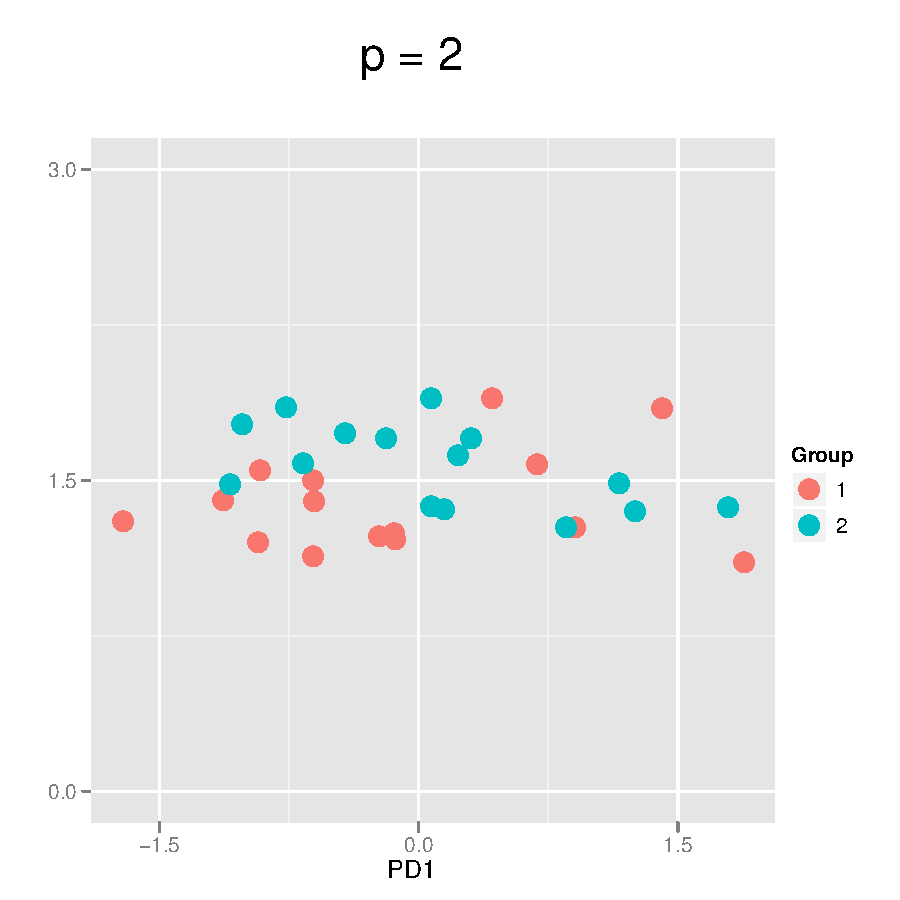
\includegraphics{plot_1d_2.pdf}}
	\scalebox{0.25}{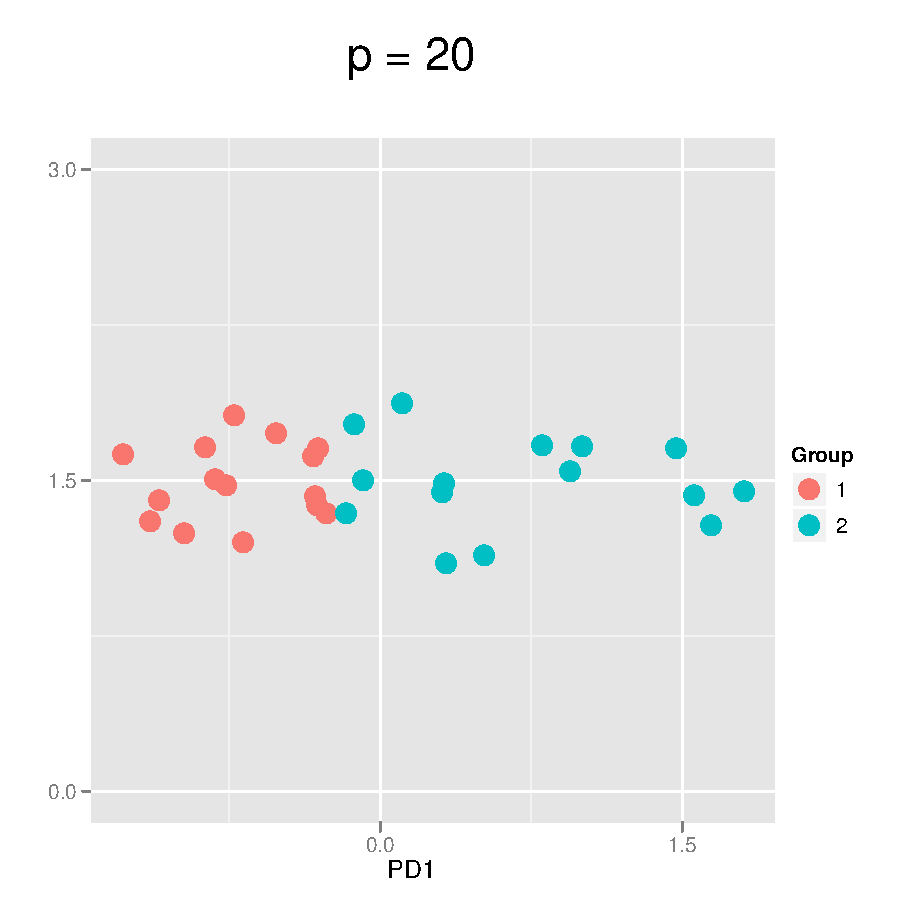
\includegraphics{plot_1d_20.pdf}}
	\scalebox{0.25}{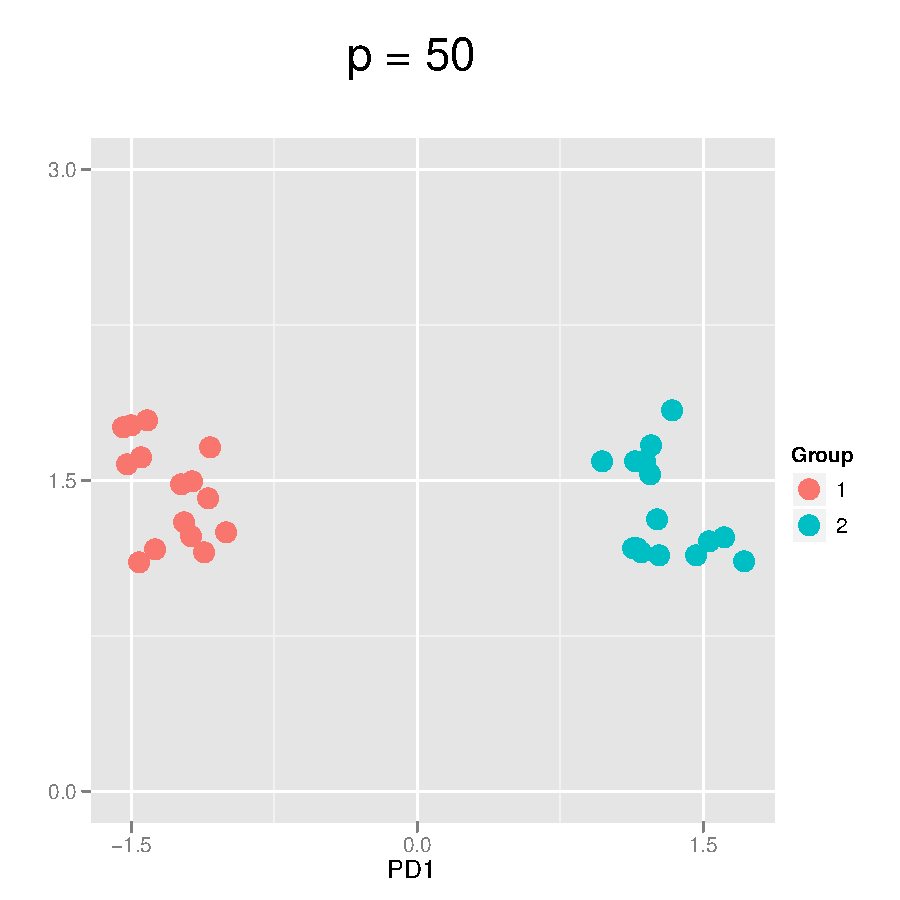
\includegraphics{plot_1d_50.pdf}}
	\scalebox{0.25}{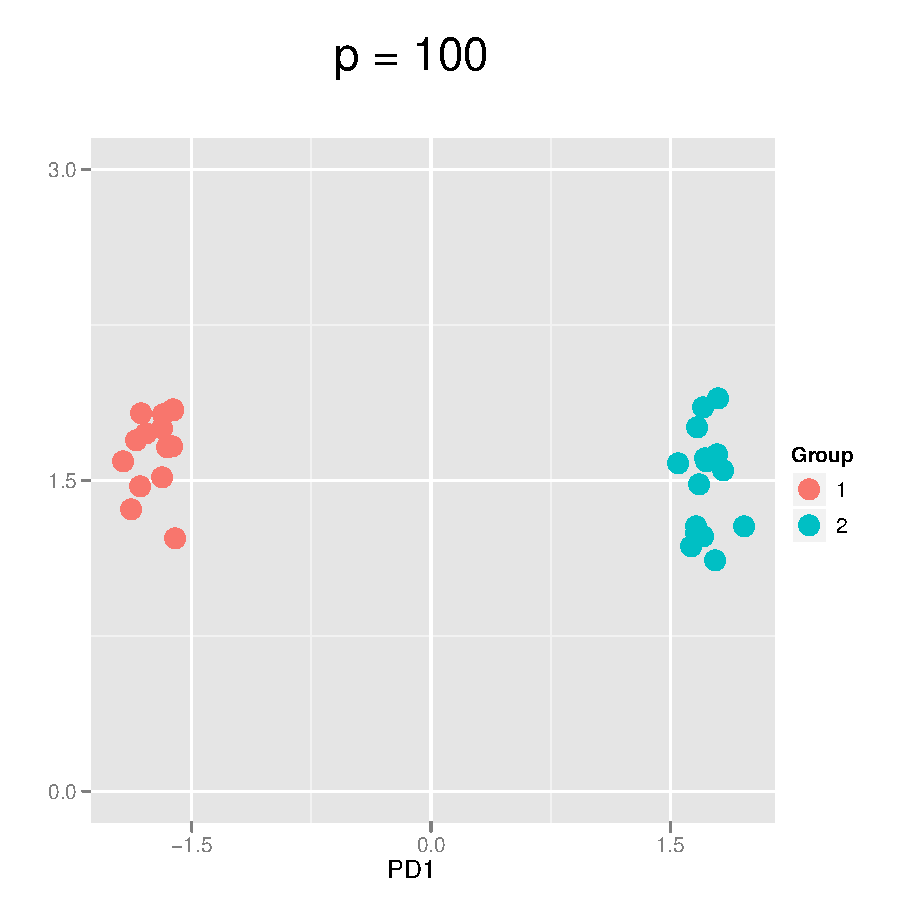
\includegraphics{plot_1d_100.pdf}}
 \scalebox{0.25}{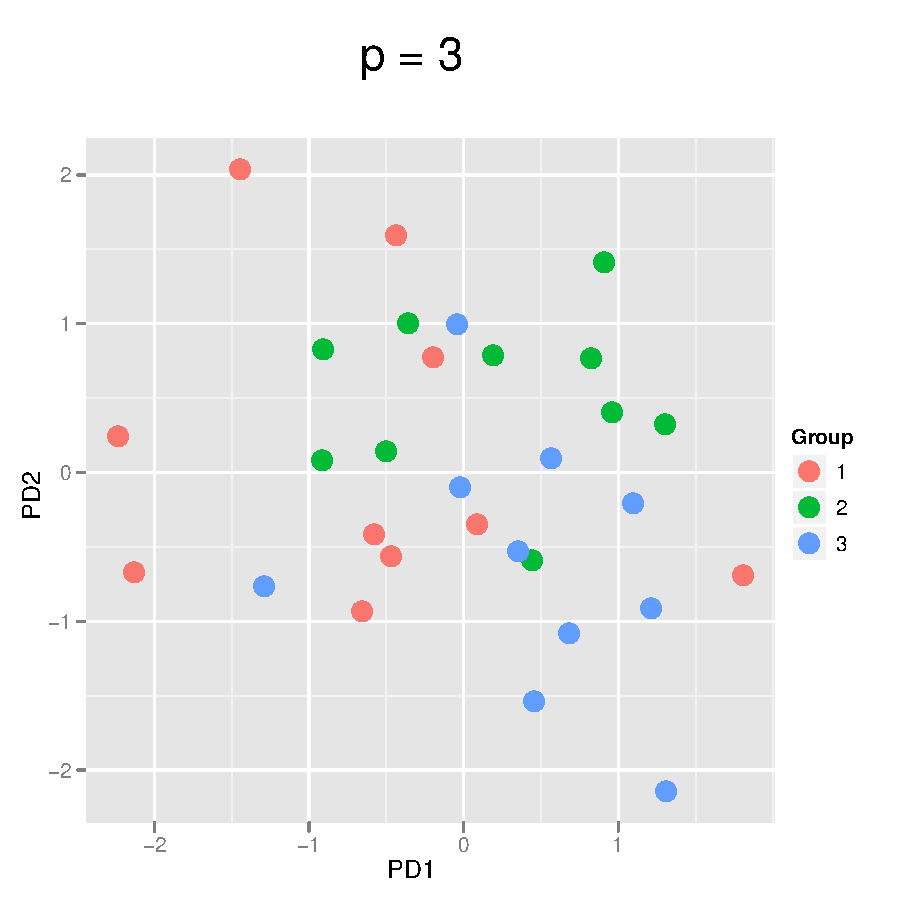
\includegraphics{plot_2d_3.pdf}}
	\scalebox{0.25}{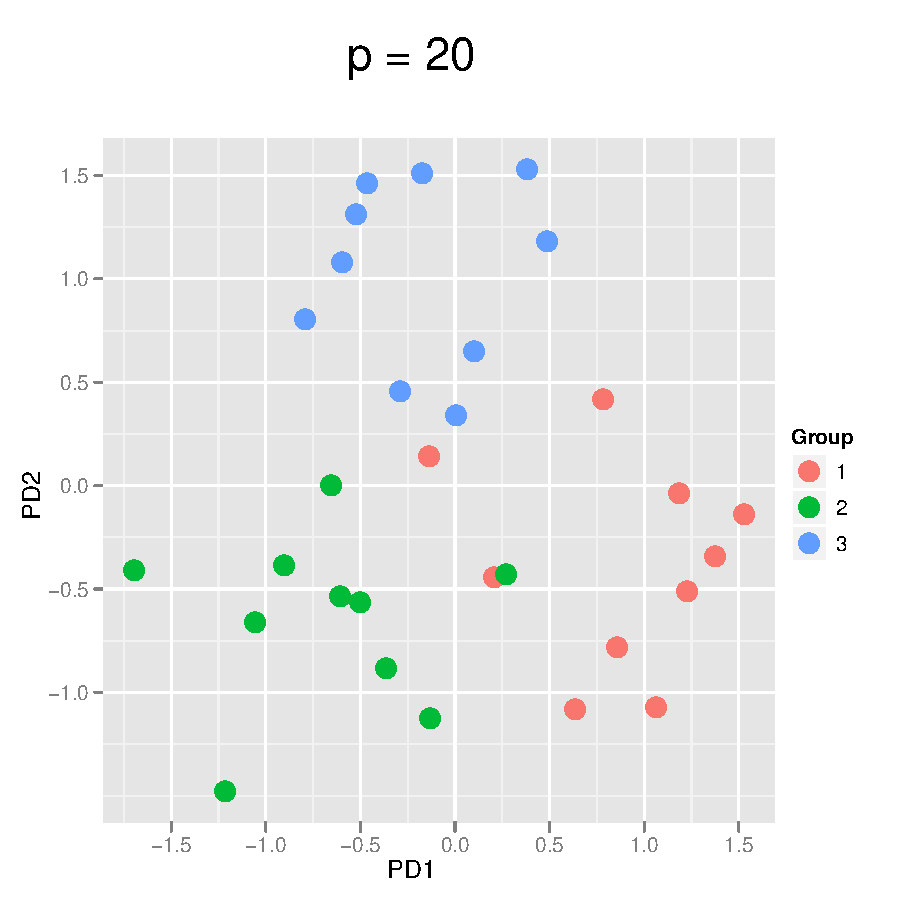
\includegraphics{plot_2d_20.pdf}}
	\scalebox{0.25}{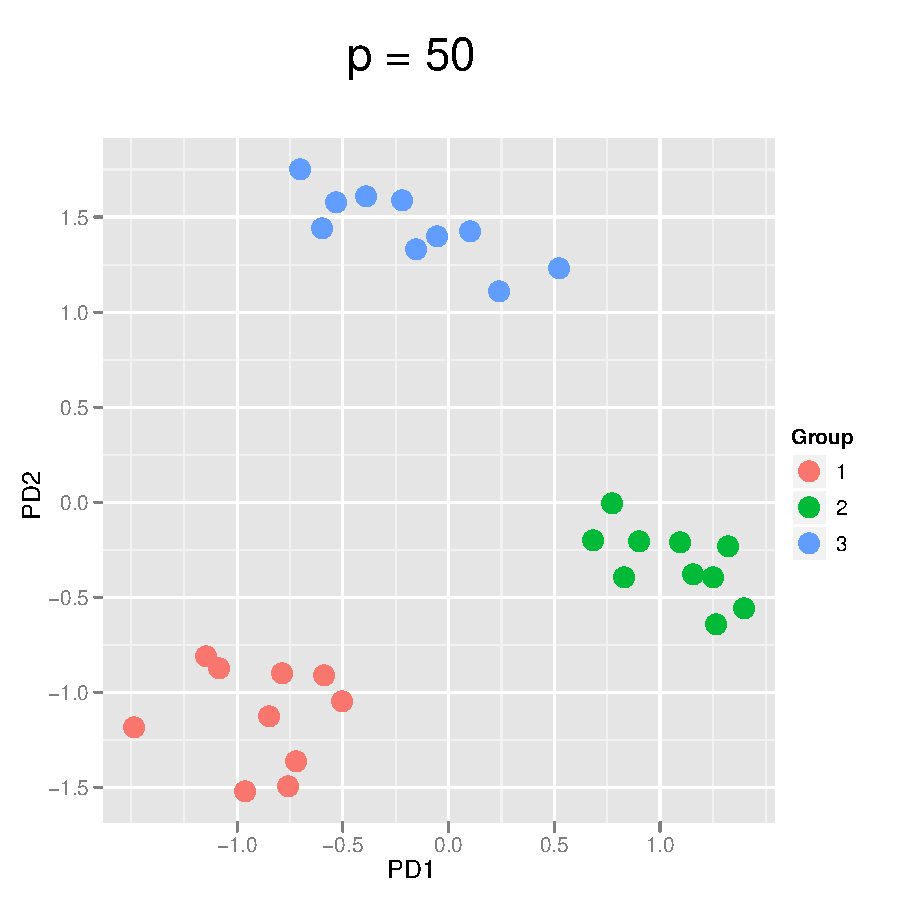
\includegraphics{plot_2d_50.pdf}}
	\scalebox{0.25}{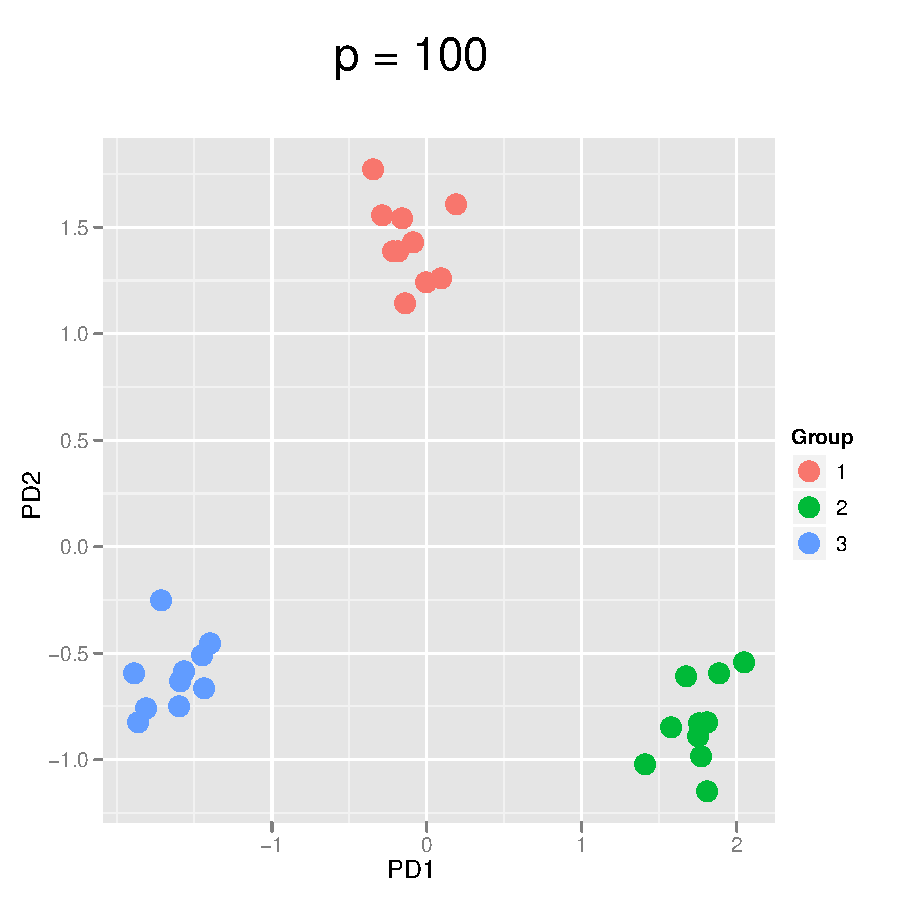
\includegraphics{plot_2d_100.pdf}}
       \caption{Plots showing one and two dimensional projections for 4 different number of dimensions $p=3$, $p=20$, $p=50$ and $p=100$. Note that the classes look more and more separated as we increase the number of dimensions when actually there is no real separation.  }
       \label{dist_1d}
\end{figure*}

%\begin{multicols}{2}
{\color{green} Description for two dimensional projections.} \\
Again consider 3 dimensions of pure noise, each dimension having 30 observations divided into 3 classes with 10 observations in each class. We again perform the projection pursuit on this and plot the two dimensional projections. Similarly, in this case the 3 colors starts separating out as we increase the number of dimensions.  Figure \ref{dist_1d} also shows the two dimensional projections for $p=3$, $p=20$, $p=50$ and $p=100$.

%\end{multicols}



%\begin{figure*}[hbtp]
%%\begin{figurehere}
%   \centering
%	\scalebox{0.25}{\includegraphics{plot-true3.pdf}}
%	\scalebox{0.25}{\includegraphics{plot-true20.pdf}}
%	\scalebox{0.25}{\includegraphics{plot-true50.pdf}}
%	\scalebox{0.25}{\includegraphics{plot-true100.pdf}}
%       \caption{Plots showing two dimensional projections for 4 different number of dimensions $p=3$, $p=20$, $p=50$ and $p=100$. Note that, like the one dimensional projections, the classes look more and more separated as we increase the number of dimensions when actually there is no real separation.  }
%       \label{dist_2d}
%\end{figure*}

%\begin{multicols}{2}


\subsection{Fun Activity}

{\color{green} The description of the procedure to calculate a probable bound for the number of dimension at which the groups start separating. } \\
The previous section clearly suggests that the clusters becomes more and more visible as we increase the number of dimensions. So a natural question is ``What is the probable dimension of data when we can clearly see the two separated clusters for the one dimensional projections and the three separated clusters for the two dimensional projections." So out of our curiosity,  we consider 2 dimensions of random noise and each dimension has 30 observations with 2 classes. Hence there is 15 observations in each class. We plot the one dimensional projections and see if we can see the classes separated. We say that the two class are separated if we can draw a straight line between the two colors without touching any of them. We repeat the same procedure by increasing the number of dimensions by 1 every time. In this manner we plot the two dimensional projections for the number of dimensions from 2 to 62. Figure \ref{conf_int} shows the plots of the one dimensional projections for the number of dimensions from 23 to 42 and Figure \ref{conf_int1} shows the plots of the two dimensional projections for $p$ ranging from 23 to 42.

%\end{multicols}

\begin{figure*}[hbtp]
%\begin{figurehere}
   \centering
       \scalebox{0.95}{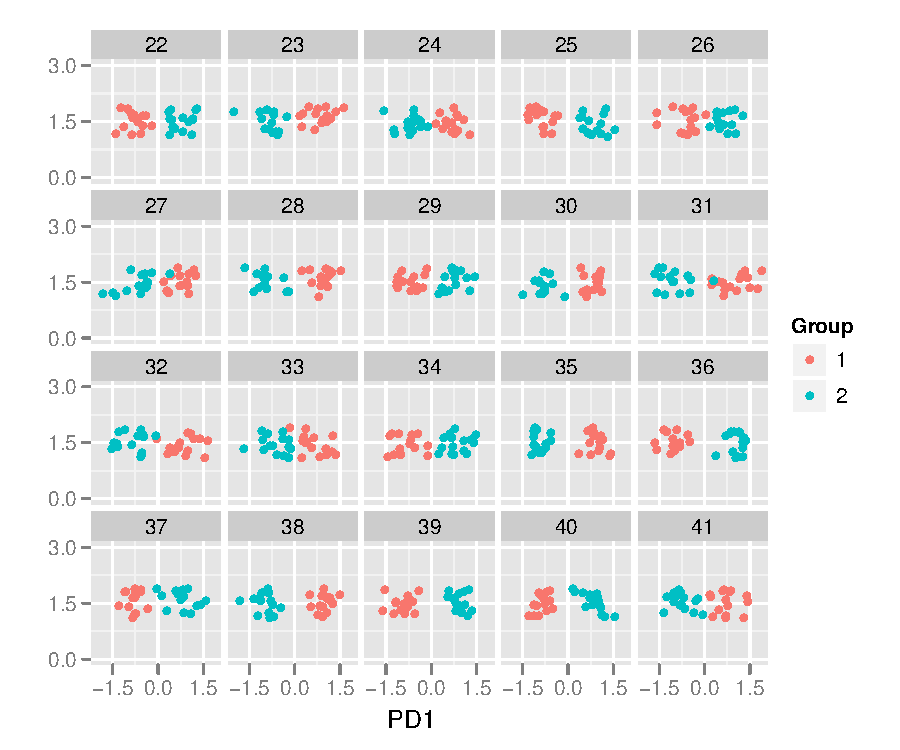
\includegraphics{plot_1d_22_41_new.pdf}}
       \caption{Plots showing the one dimensional projections for a fixed sample size $n=30$ and the number of dimensions ranging from 23 to 42. The number written above the plot is the number of dimension. Can you see where the colors starts separating?  }
       \label{conf_int}
\end{figure*}

\begin{figure*}[hbtp]
%\begin{figurehere}
   \centering
       \scalebox{0.95}{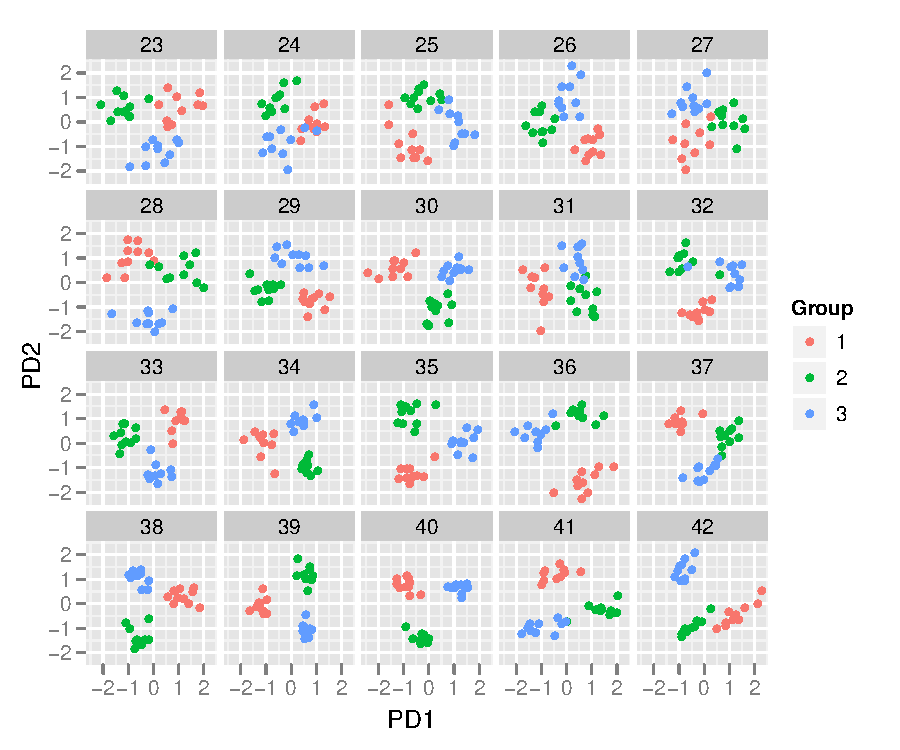
\includegraphics{plot_2d_23_42_new.pdf}}
       \caption{Plots showing the two dimensional projections for a fixed sample size $n=30$ and the number of dimensions ranging from 23 to 42. The number written above the plot is the number of dimension. Can you see where the colors starts separating?  }
       \label{conf_int1}
\end{figure*}

%\begin{multicols}{2}
 
Now we see the plot where the one dimensional projections shows a separation between the colors. We draw 100 such plots and note the number of dimension at which the classes separate out. We take the 5th and the 95th percentile of these numbers to obtain a probable range of the dimension at which the clusters are formed.

Similarly we take 3 dimensions of pure noise with 30 observations in each dimension. Each dimension is divided into 3 classes, with 10 observations in each class. We plot the two dimensional projections and see whether the classes are separated. We again define the classes to be separate if we can draw three lines making an angle of $120^{\circ}$ among themselves without touching any color. So the classes will be separated if none of the colors overlap. We again repeat the same procedure by increasing the number of dimensions by 1 every time. We plot the two dimensional projections from 3 to 62 for sample size 30. We again make 100 such plots and note the number of dimension at which the classes start separating. 

{\color{green} Explanation of the findings. } \\
Hence a probable range that we obtain from the 100 plots for the one dimensional projection is between 24 and 34 and the a probable range for the two dimensional projection is between 26 and 36. 

\section{Conclusions}
{\color{green} Concluding remarks summarizing the different findings.} \\
The purpose of this paper has been to utilize  visual inference methods to examine the reliability of the projection pursuit results. We found that there were no problems with the projection pursuit: that viewers had more difficulty picking the ``true" data when it was pure noise. We also use the visual inference method to examine when clusters start to form for a large number of dimensions of pure noise for a fixed sample size. The classes are more and more separated as we increase the number of dimensions. Being motivated by the separation of the classes, we looked for a probable range of the number of dimensions at which the classes start separating for both one dimensional and two dimensional projections, in order to compare with the theoretical predictions. These were between 24-34 for one dimensional projections, and 26-36 for two dimensional projections.

\paragraph{Acknowledgement:}
%
This work was funded by National Science Foundation grant DMS 1007697.

\bibliographystyle{plainnat}
%%\bibliographystyle{ieeetr}
\bibliography{references}

\end{document}
